%% ----------------------------------------------------------------
%% Thesis.tex -- MAIN FILE (the one that you compile with LaTeX)
%% ---------------------------------------------------------------- 

% Set up the document
\pdfminorversion=7
\documentclass[a4paper, 11pt, oneside]{Thesis}  % Use the "Thesis" style, based on the ECS Thesis style by Steve Gunn
\graphicspath{Figures/}  % Location of the graphics files (set up for graphics to be in PDF format)

% Include any extra LaTeX packages required
\usepackage[square, numbers, comma, sort&compress]{natbib}  % Use the "Natbib" style for the references in the Bibliography
\usepackage{verbatim}  % Needed for the "comment" environment to make LaTeX comments
\usepackage{vector}  % Allows "\bvec{}" and "\buvec{}" for "blackboard" style bold vectors in maths
\usepackage{acronym}
\usepackage[final]{pdfpages}
%\usepackage[hidelinks]{hyperref}
%\hypersetup{colorlinks=false}  % Colours hyperlinks in blue, but this can be distracting if there are many links.
\hypersetup{
    colorlinks,
    linkcolor={red!50!black},
    citecolor={blue!50!black},
    urlcolor={blue!80!black}
}
%% ----------------------------------------------------------------
\begin{document}
\frontmatter      % Begin Roman style (i, ii, iii, iv...) page numbering

% Set up the Title Page
\title{Machine Learning Based Restaurant Location Analysis in Hamburg}
\authors  {
			\texorpdfstring
            {\href{}{Hung Viet Hu}}
            {Hung Viet Hu}, 
			\texorpdfstring
            {\href{}{Sachin Kumar}}
            {Sachin Kumar}, 
			\texorpdfstring
            {\href{https://www.linkedin.com/in/vincent-meyer-zu-wickern-705b9610a/}{Vincent Meyer zu Wickern}}
            {Vincent Meyer zu Wickern}
            }
            
            
\addresses  {\groupname\\\deptname\\\univname}  % Do not change this here, instead these must be set in the "Thesis.cls" file, please look through it instead
\date       {\today}
\subject    {}
\keywords   {}

\maketitle
%% ----------------------------------------------------------------

\setstretch{1.5}  % It is better to have smaller font and larger line spacing than the other way round

% Define the page headers using the FancyHdr package and set up for one-sided printing
\fancyhead{}  % Clears all page headers and footers
\rhead{\thepage}  % Sets the right side header to show the page number
\lhead{}  % Clears the left side page header

\pagestyle{fancy}  % Finally, use the "fancy" page style to implement the FancyHdr headers

%% ----------------------------------------------------------------
% Declaration Page required for the Thesis, your institution may give you a different text to place here
%\Declaration{

\addtocontents{toc}{\vspace{1em}}  % Add a gap in the Contents, for aesthetics
We declare that this paper and the work presented in it are our own. We confirm that:

\begin{itemize} 
\item[\tiny{$\blacksquare$}] This work was done wholly or mainly while in candidature for a research degree at this University.
 
\item[\tiny{$\blacksquare$}] Where any part of this paper has previously been submitted for a degree or any other qualification at this University or any other institution, this has been clearly stated.
 
\item[\tiny{$\blacksquare$}] Where we have consulted the published work of others, this is always clearly attributed.
 
\item[\tiny{$\blacksquare$}] Where we have quoted from the work of others, the source is always given. With the exception of such quotations, this paper is entirely my own work.
 
\item[\tiny{$\blacksquare$}] We have acknowledged all main sources of help.
 
\item[\tiny{$\blacksquare$}] Where the paper is based on work done by ourselves jointly with others, we have made clear exactly what was done by others and what we have contributed ourselves.
\\
\end{itemize}
 
 
Signed:\\
\rule[1em]{25em}{0.5pt}  % This prints a line for the signature
 
Date:\\
\rule[1em]{25em}{0.5pt}  % This prints a line to write the date

Signed:\\
\rule[1em]{25em}{0.5pt}  % This prints a line for the signature
 
Date:\\
\rule[1em]{25em}{0.5pt}  % This prints a line to write the date

Signed:\\
\rule[1em]{25em}{0.5pt}  % This prints a line for the signature
 
Date:\\
\rule[1em]{25em}{0.5pt}  % This prints a line to write the date
\clearpage  % Declaration ended, now start a new page

%% ----------------------------------------------------------------
% The "Funny Quote Page"
%\pagestyle{empty}  % No headers or footers for the following pages
%
%\null\vfill
%% Now comes the "Funny Quote", written in italics
%\textit{``Write a funny quote here.''}
%
%\begin{flushright}
%If the quote is taken from someone, their name goes here
%\end{flushright}
%
%\vfill\vfill\vfill\vfill\vfill\vfill\null
%\clearpage  % Funny Quote page ended, start a new page
%% ----------------------------------------------------------------

% The Abstract Page
\addtotoc{Abstract}  % Add the "Abstract" page entry to the Contents
\abstract{
\addtocontents{toc}{\vspace{1em}}  % Add a gap in the Contents, for aesthetics


}

\clearpage  % Abstract ended, start a new page
%% ----------------------------------------------------------------

\setstretch{1.5}  % Reset the line-spacing to 1.3 for body text (if it has changed)

% The Acknowledgements page, for thanking everyone
%\acknowledgements{
%\addtocontents{toc}{\vspace{1em}}  % Add a gap in the Contents, for aesthetics

%The acknowledgements and the people to thank go here, don't forget to include your project advisor\ldots

%}
%\clearpage  % End of the Acknowledgements
%% ----------------------------------------------------------------

\pagestyle{fancy}  %The page style headers have been "empty" all this time, now use the "fancy" headers as defined before to bring them back


%% ----------------------------------------------------------------
\lhead{\emph{Contents}}  % Set the left side page header to "Contents"
\tableofcontents  % Write out the Table of Contents

%% ----------------------------------------------------------------
\lhead{\emph{List of Figures}}  % Set the left side page header to "List if Figures"
\listoffigures  % Write out the List of Figures

%% ----------------------------------------------------------------
%\lhead{\emph{List of Tables}}  % Set the left side page header to "List of Tables"
%\listoftables  % Write out the List of Tables

%% ----------------------------------------------------------------
\setstretch{1.5}  % Set the line spacing to 1.5, this makes the following tables easier to read
\clearpage  % Start a new page
\lhead{\emph{Abbreviations}}  % Set the left side page header to "Abbreviations"
\btypeout{Abbreviations}
\chapter{Abbreviations}


\begin{acronym}
\acro{alkis}[ALKIS\copyright]{Amtliches Ligenschaftskatasterinformationssystem (Authoritative Real Estate Cadastre Information System)}
\acro{ascii}[ASCII]{American Standard Code for Information Interchange}
\acro{crs}[CRS]{Cordinate Reference system}
\acro{csv}[CSV]{comma-separated values}
\acro{etrs89}[ETRS89]{European Terrestrial Reference System 1989}
\acro{metaver}[MetaVer\copyright]{MetadatenVerbund}
\acro{sse}[SSE]{sum of squared errors of the regression model}
\acro{sst}[SST]{sum of squred errors of the baseline model}
\acro{wms}[WMS]{Web Map Service}

\end{acronym}

%% ----------------------------------------------------------------
%\clearpage  % Start a new page
%\lhead{\emph{Physical Constants}}  % Set the left side page header to "Physical Constants"
%\listofconstants{lrcl}  % Include a list of Physical Constants (a four column table)
{
% Constant Name & Symbol & = & Constant Value (with units) \\
%Speed of Light & $c$ & $=$ & $2.997\ 924\ 58\times10^{8}\ \mbox{ms}^{-\mbox{s}}$ (exact)\\

}

%% ----------------------------------------------------------------
%\clearpage  %Start a new page
%\lhead{\emph{Symbols}}  % Set the left side page header to "Symbols"
%\listofnomenclature{lll}  % Include a list of Symbols (a three column table)
{
% symbol & name & unit \\
%$a$ & distance & m \\
%$P$ & power & W (Js$^{-1}$) \\
%& & \\ % Gap to separate the Roman symbols from the Greek
%$\omega$ & angular frequency & rads$^{-1}$ \\
}
%% ----------------------------------------------------------------
% End of the pre-able, contents and lists of things
% Begin the Dedication page

\setstretch{1.3}  % Return the line spacing back to 1.3

%\pagestyle{empty}  % Page style needs to be empty for this pagef
%\dedicatory{For/Dedicated to/To my\ldots}

\addtocontents{toc}{\vspace{2em}}  % Add a gap in the Contents, for aesthetics


%% ----------------------------------------------------------------
\mainmatter	  % Begin normal, numeric (1,2,3...) page numbering
\pagestyle{fancy}  % Return the page headers back to the "fancy" style

% Include the chapters of the thesis, as separate files
% Just uncomment the lines as you write the chapters

\chapter{Introduction}
\lhead{\emph{Introduction}}

\chapter{Elements of a restaurant location analysis}
\lhead{\emph{Elements of a restaurant location analysis}}


\chapter{Data Sources}
\lhead{\emph{Data Sources}}


\section{Transparency Portal Hamburg}
As the first German federal state, Hamburg enacted a transparency law on October 6, 2012 \cite{Murjahn.2016}. Opposed to a right to request information, which all citizens had until this date, a new duty to inform the public was laid upon the state’s administration offices. All information that would fall under this law, now had to to be published in a freely available standard format on a centered storage of information. The single pieces of information, which would fall under the law, varied highly in precision and the comprehensive term of ``geodata'' was requested opposed to precise datasets of geodata. A legal interpretation was worked out for all requested points and a plan for the release of geodata was designed consisting of the basic data for measurement admistration and the technical geodata for special administration offices. The transparency law granted a period of two years for the technical implementation.

In October 2014, the ``Transparency Portal'' (http://transparenz.hamburg.de/) as the major component of the implementation of the transparency law was released \cite{Murjahn.2016}. With this portal, the Hamburg citizens have a multitude of data and documents available that was prior only available to Hamburg's administration. One important focus was the release of geodata that was even before the law in preparation for an ``Open GeoData'' model. In this ``Open GeoData'' model, geodata was split into two groups of data sets, one group extractable with little effort, but free to the public and expected with a high use, and another group with expected high demand and high revenue on the sale of this data. For this second group of datasets, more effort with new measurements had to be arranged. With the transparency law in place, all datasets were merged into the Transparency Portal and yielded a much higher download count than the count of dataset sales before the portal was active. The Transparency Portal uses a standardized meta data repository called the \ac{metaver} in collaboration with other German federal states.

\section{Online Restaurant Portals}

\subsection{Other potential restaurant portals}

tripadvisor is one of the biggest rating portals for travel and travel related businesses, such as restaurants, with cumulated 600 million reviews and opinions until 2017 \cite{StephenKaufer.27.04.2018}. This made tripadvisor a potential portal for the analysis of restaurant reviews to extract data from. However, it was found that any scraping, download or copy of the data with automated or manual methods is legally prohibited from tripadvisor, which excluded tripadvisor as a data basis for the analysis of this paper.

Google 



\subsection{Yelp}
 
 \chapter{Analysis Methods}
\lhead{\emph{Analysis Methods}}

\section{Random Forest Regression}

\section{Regression Performance Measures}

A common performance measure for the quality of fit of regression models is the ``coefficient of determination'', which is also called ``R-Squared'' \cite{Devasthali.2018}. This coefficient of determination uses a baseline model, which is a model that consistently predicts the mean of all observations of the dependent variable. This baseline model is a model that a created regression model can be compared to, to see how much more accurate the own predictions were to a poor model.

Following are the calculation of the \ac{sse}, \ac{sst} and R-squared \cite{Devasthali.2018}:

\[SSE = \sum\limits_{i=1}^n (y_{i} - \hat{y}_{i})^2\]

\[SST = \sum\limits_{i=1}^n (y_{i} - \hat{y}_{i})^2\]

\[ R^2 = 1 - \frac{SSE}{SST}\]

According to this calculation, R-squared always lies between 0 and 1, if the created regression model yields more accurate predictions than the baseline model \cite{Devasthali.2018}. The closer R-squared is to 1, the closer are the predictions by the regression model to the actual values. Additionally, the higher R-squared is, the more variations of the dependent variable are explained by the model.

A weak point of R-squared is that additions of more independent variables never lower the value of R-squared, even for variables with little or no information gain \cite{Devasthali.2018}. To cope with this problem, another performance measure called ``adjusted R-squared'' was introduced, which introduces a negative effect on the measure for the inclusion of ineffective variables. It is calculated as follows \cite{Devasthali.2018}:

\[ \bar{R}^2 = 1 - (1-R^2)\frac{n-1}{n-p-1}\]

n = no of data points

p = no of independent variables in the model

R-squared therefore only improves (moves closer to 1), if significant variables are added to the model and deteriorates (moves closer to 0), if variables are added that are not valuable to the prediction of the dependent variable \cite{Devasthali.2018}. 

\chapter{Data Extraction}
\lhead{\emph{Data Extraction}}

\section{Hamburg District Map}

Since usually cities raise important figures in aggregation per admistrative area, in Hamburg being the single city districts, these administrative areas should be imported into QGIS to be able to link single restaurants to an administrative area and hence figures that could be important as dependent variables to predict restaurant success. The borders of the administrative areas are taken from a dataset of the Transparency Portal called ``ALKIS Verwaltungsgrenzen Hamburg'' \cite{LandesbetriebGeoinformationundVermessung.28.02.2018}. This dataset is available in multiple dataformats, is reported to have a 0\% data deficit and a precision of 0.1 meters. It is part of the \ac{alkis}, a digital combination of the real estate book information and a real estate map \cite{ALKIS2019}.

For this analysis, the GML version of the administrative boundaries were downloaded and imported to QGIS. Loading the administrative boundaries into QGIS, the \ac{etrs89} \ac{crs} defined by EPSG:25832 was selected, as was defined in the metadata of the dataset. All following elements that are loaded into QGIS are as well projected in this \ac{crs}. The imported boundaries can be seen in figure \ref{fig:administrative_boundaries}.

\begin{figure}[h]
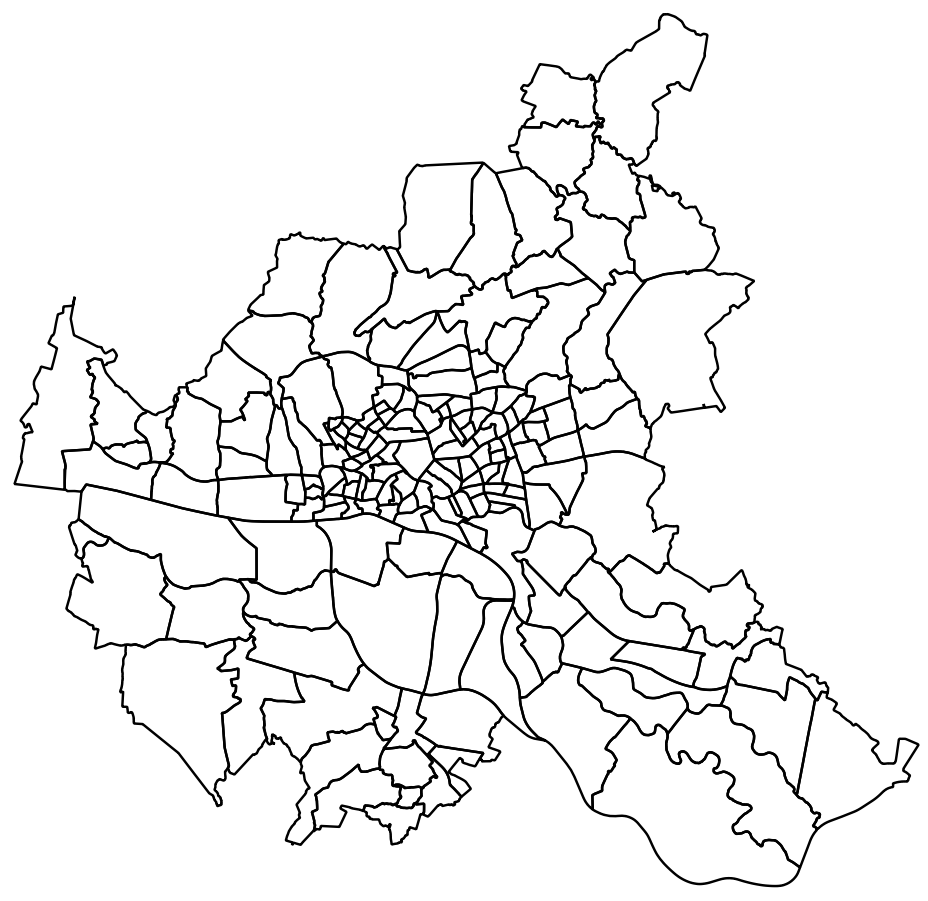
\includegraphics[scale=0.5]{Figures/Hamburg_Administrative_Boundaries.png}
\centering
\caption{Administrative boundaries of Hamburg in QGIS}
\label{fig:administrative_boundaries}
\end{figure}


\section{Yelp Restaurant Data Extraction}



\subsection{Restaurant Success Calculation}

The success of a restaurant is usually measured by financial figures, such as revenue, profit or business growth. However, this information is not publicly available for all small businesses, so a restaurant success has to be assumed from other metrics. Other metrics are important to businesses today are online reviews and ratings. They may influence the success of a restaurant and as well may mirror a restaurant's success. In fact, the rating and reviews a restaurant displays on a portal such as Yelp are their display of success to their customers on the Internet, for which reason the success measures in this paper should combine the two figures of review count and average rating.

The average rating and review count have been standardized to set them to a comparable range of values while still keeping the effects of outliers. The standardization has been conducted with the StandardScaler function of the scikitlearn-preprocessing package. Having the average rating and review count in comparable ranges the values were added and saved into a success variable to value them equally in their part of the success. The success, hence, is the sum of the standardized Yelp review count and average rating. In figure \ref{fig:restaurant_success_distribution}, the distribution of the success values can be seen, they are in the range between ca. 4.2 and 1ca. 13.30.

\begin{figure}[h]
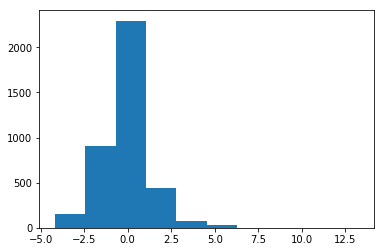
\includegraphics[scale=0.5]{Figures/restaurant_success_distribution.png}
\centering
\caption{Distribution of Restaurant Success Values}
\label{fig:restaurant_success_distribution}
\end{figure}


\section{City District Profiles Hamburg}

In this study, it was considered that the city district that a restaurant was located in, may have an influence on the success of this restaurant, e.g. through direct or indirect effects from the demographics in this district. Therefore, ``city part profiles'' published in the Transparency Portal of Hamburg were taken into account \cite{Profiles2018}. The dataset presents structure data for all of Hamburg's city parts for the topic areas of population, living, council elections, social structure, infrastructure and traffic. The last dataset was published on the 19.03.2018, but dated back to data from 2016.

The data was available in XLSX-format, in which it was downloaded. Afterwards, the formatting was adjusted to be able to save the content as a csv. With this CSV, all the necessary information, that would later be used in the analysis, was available as a spreedsheet that could be loaded into Python.

\section{Proximity to Water}

As Hamburg is an important port city and almost 10\% of the city is covered by the habor \cite{HamburgStadt2019}, water is an important consideration in the analysis of restaurant success. To know the water locations in hamburg is important, because restaurants are regularly not placed on water (restaurant boats are not condidered as potential location candidates for simplicity). Additionally, water may influence the success of a restaurant with customers who may like to sit with a water view. Out of these reasons, the locations of water in Hamburg should be made out and the proximity of each restaurant to the next water location should be calculated.

For the extraction of water location, a geological ground map of Hamburg in the scale 1:5,000 \cite{GeologischeKarte2019} was added as a \ac{wms} layer into QGIS, as depicted in figure \ref{fig:geologische_karte}. The dark blue color on this WMS layer indicates that an area is on water ground, e.g. a river. Since the water spots on WMS layer were not able to be processed as measurable points, yet, these had to be preprocessed before. 

\begin{figure}[h]
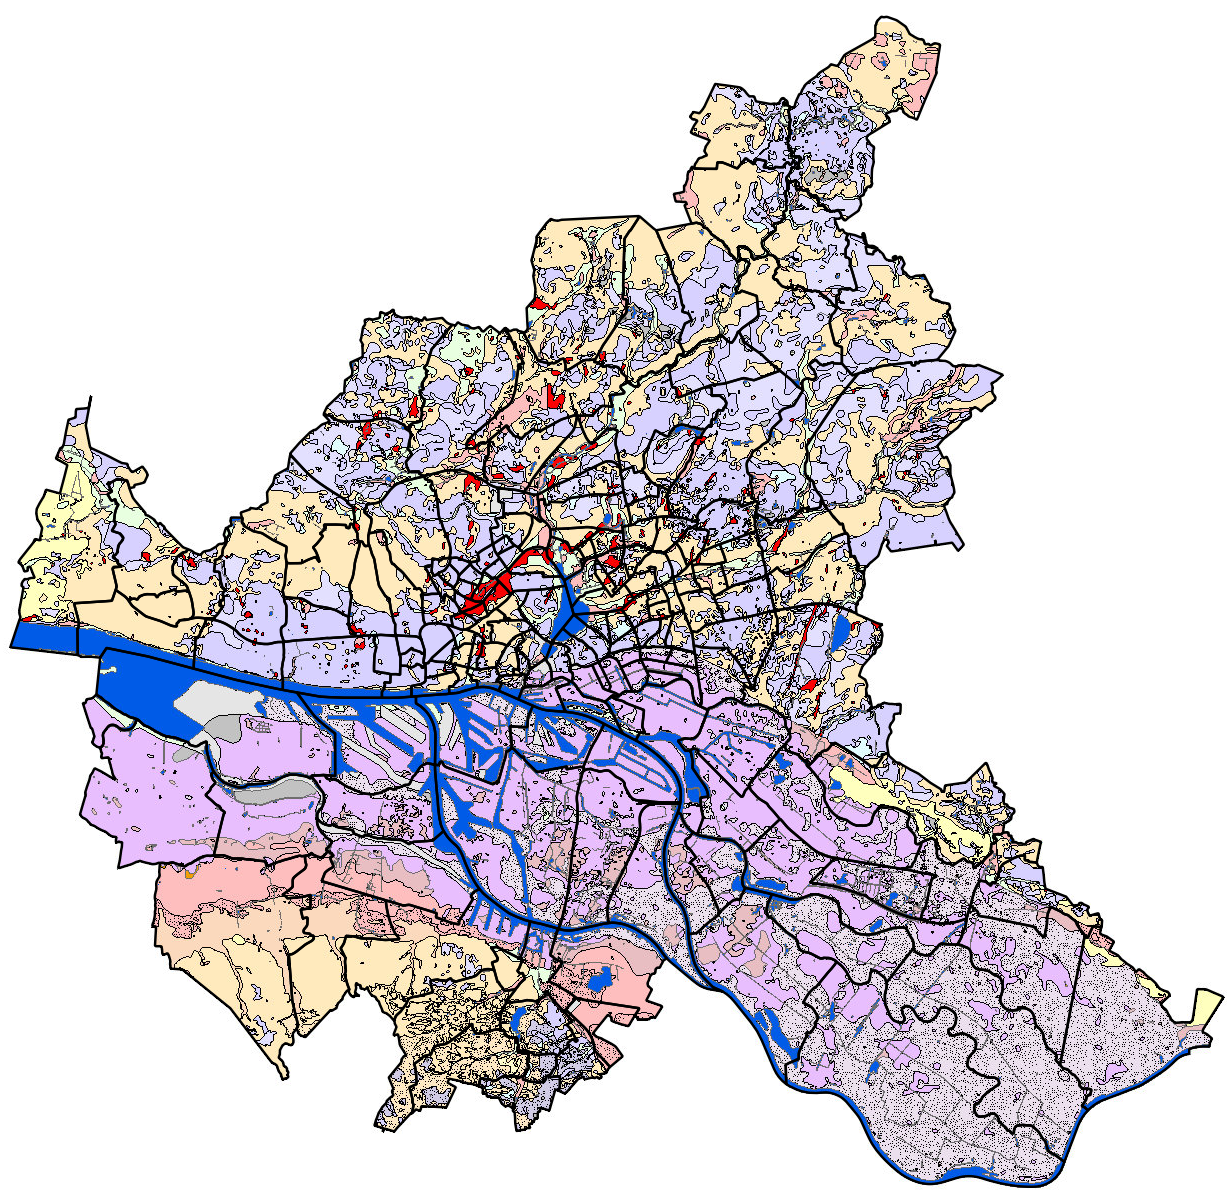
\includegraphics[scale=0.5]{Figures/WMS_Layer_Geologische_Karte.png}
\centering
\caption{WMS Layer ``Geologische Karte Hamburg''}
\label{fig:geologische_karte}
\end{figure}

In the first step, the \ac{wms} map was saved as a raster with the ``Save as...'' option of QGIS. The output was set to a ``Rendered Image'' in Format ``GTiff''. The \ac{crs} stays \ac{etrs89} and the resolution is first set to 100\%, described by entering a 1 into both horizontal and vertical resolution. A new raster file is created.

The newly created raster file had a high resolution and needed to be reduced to be processed further. The resolution was reduced by conducting the QGIS raster conversion function ``Translate (Convert format)''. In the upcoming dialog, the ``outsize'' resolution was set to 3\% and the output location was set to a new GeoTIFF file. In the created execution code in the buttom of the dialog, the standard ``of''-parameter ``GMT'' had to be changed to ``GTIFF''. The resolution was after the reolution reduction still adquate to present the water areas.

In the third step, the new and reduced raster file was converted into a grid that would store a certain color value for each of the points on the raster together with their coordinates. This could be conducted by using the same QGIS conversion function ``Translate (Convert format)'' as in the previous step, however, in the corresponding dialog, the ``outsize'' resolution was not touched and the ouput format was set to an \ac{ascii} gridded XYZ file. In the generated XYZ-grid, a delimited value storage of three attributes per record could be found. The first two attributes present the x and y values on the \ac{etrs89} \ac{crs} and the third value a value for the colors with their luminosity is stored. The luminosity ``0'' is the darkest value in the grid and marks the prior dark blue water locations. This knowledge was used in a python script that was implemented to create a new dataset by looping through every record in the grid and to only keep the records, in which the luminosity would match ``0''. Thereby only water locations would be part of the new dataset.

The fourth step consisted of the calculation of the distances of each restaurant to the next water spot by using a Python script. In this script, all restaurants and water locations were loaded into the memory. Then, for each restaurant, the lowest distace to water was calculated by looping through all water points and calculating the Euclidian distance to them. At the end, a minimum water distance was found for each restaurant that was stored together with the restaurant ID in a \ac{csv}-file for the use in analysis.








\chapter{Machine Learning}
\lhead{\emph{Machine Learning}}

\section{Exploratory Data Analysis}

\section{Data Preprocessing}

\subsection{Handling of Missing Values}

\subsection{Feature Subset Selection}

\subsection{Dimensionality Reduction}

\section{Data Analysis}


\chapter{Results and Discussion}
\lhead{\emph{Results and Discussion}}

\section{Results}

\section{Discussion}

\chapter{Conclusion}
\lhead{\emph{Conclusion}}  



%% ----------------------------------------------------------------
% Now begin the Appendices, including them as separate files

%\addtocontents{toc}{\vspace{2em}} % Add a gap in the Contents, for aesthetics

%\appendix % Cue to tell LaTeX that the following 'chapters' are Appendices

%\input{Appendices/AppendixA}	% Appendix Title

%\input{Appendices/AppendixB} % Appendix Title

%\input{Appendices/AppendixC} % Appendix Title

\addtocontents{toc}{\vspace{2em}}  % Add a gap in the Contents, for aesthetics
\backmatter

%% ----------------------------------------------------------------
\label{Bibliography}
\lhead{\emph{Bibliography}}  % Change the left side page header to "Bibliography"
\bibliographystyle{unsrtnat}  % Use the "unsrtnat" BibTeX style for formatting the Bibliography
\bibliography{Bibliography}  % The references (bibliography) information are stored in the file named "Bibliography.bib"

\end{document}  % The End
%% ----------------------------------------------------------------